\chapter{Related Work}\label{cha:related}
In this chapter work related to physics simulations and GPU based solutions are
presented.
\section{Spherical decomposition}\label{sec:decomp}
\cite{gpugems} presents a method for collision detection and response using spherical
decomposition. By subdividing the object into a collection of spheres one gets an
approximation of the shape. Since each new collision shape is locally convex, collision
detection is much simplified, but the global result of the decomposition still has
concave properties. Since each new collision shape is the same primitive, only
one type of collision detection and response is needed; in this case spheres.
For an example of objects
decomposed in this manner, see figure~\ref{fig:bunnies}.

\begin{figure}[H]
  \centering
  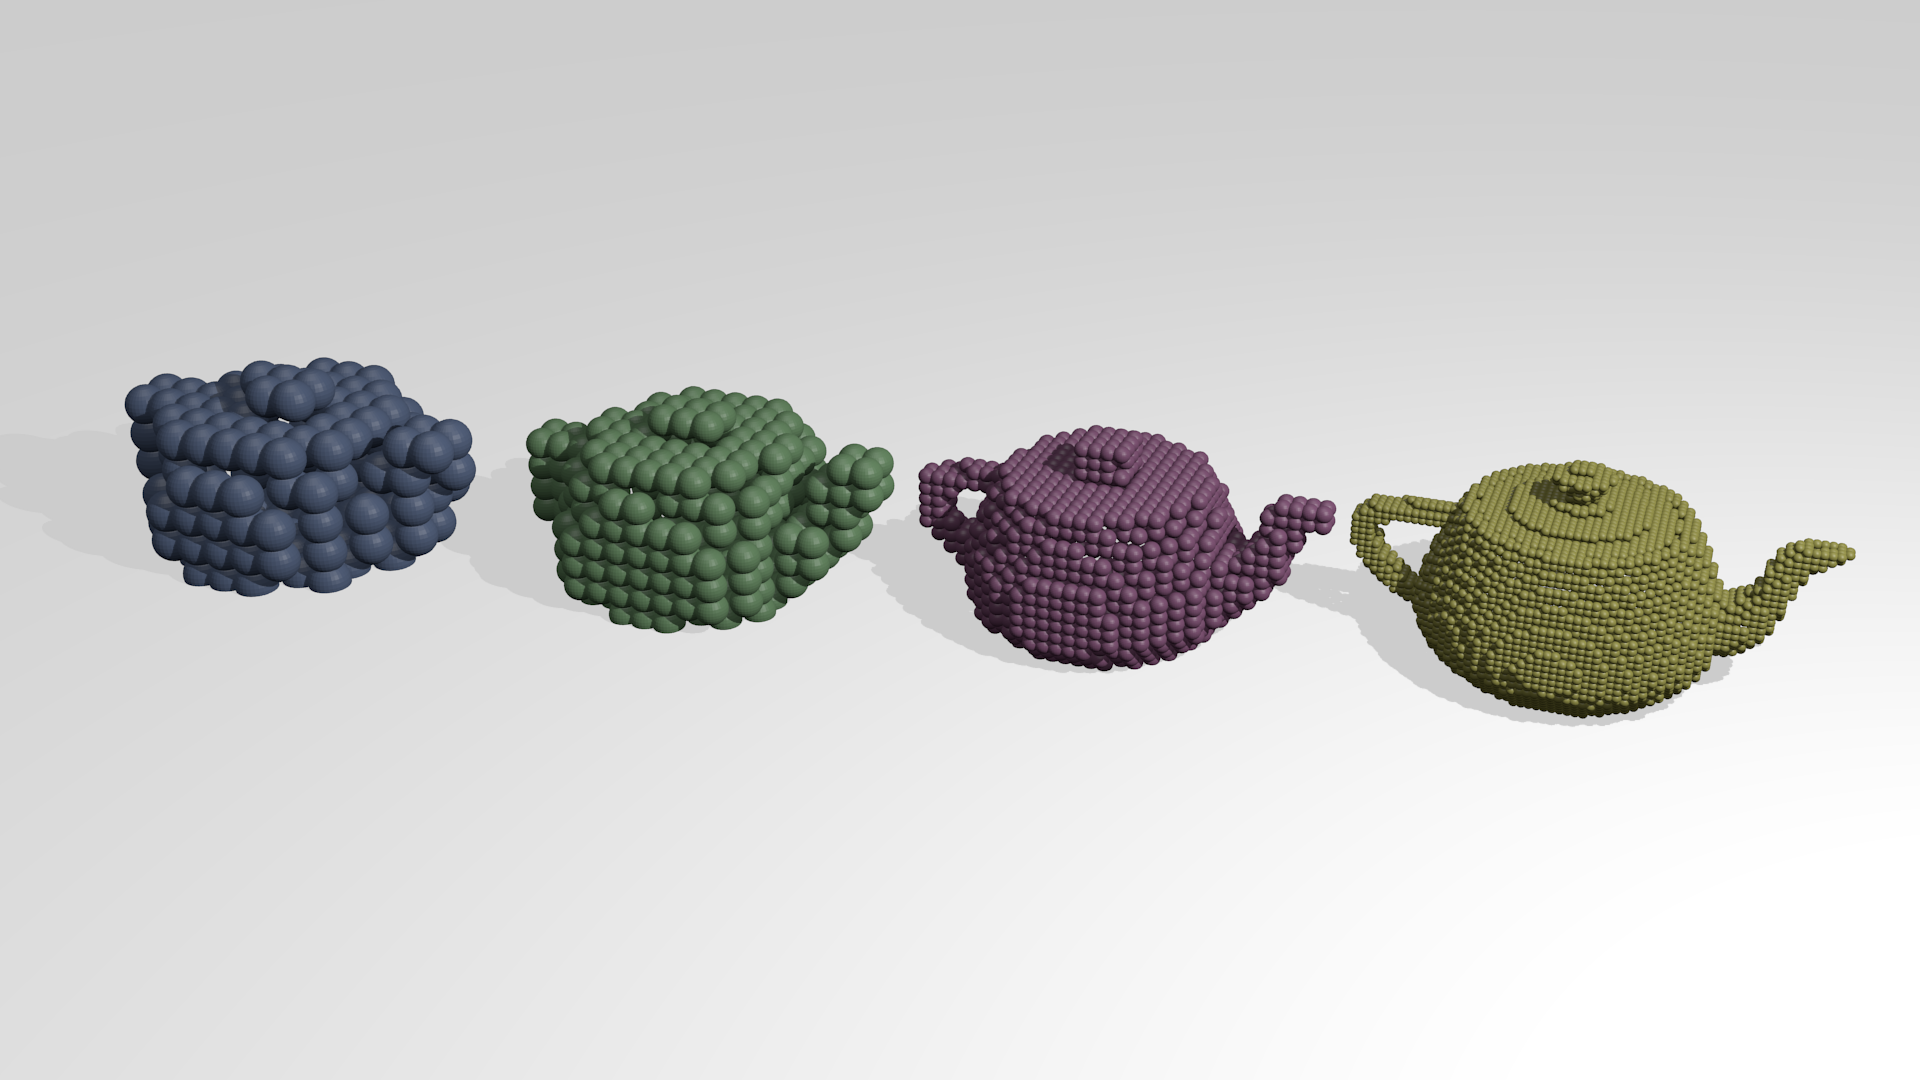
\includegraphics[width = 0.9\textwidth]{voxelExample.png}
  \caption{Varying degrees of spherical decomposition of the Utah Teapot}
  \label{fig:bunnies}
\end{figure}

\subsection{Spring-damper model}
The spring-damper model is a model for collision response described in~\cite{gpugems} and by~\cite{fossum}.
This model has the benefit of being quite easy to implement on both CPU and GPU.
However, since there are two design parameters, the spring constant and the damping
constant, the system can be difficult to tune. Often a parameter constellation that works
well for one system will fail for another.

The equations below describe how the force and torque can be derived for this type
of model. The equations describe the forces for collision between sphere $i$ and $j$,
where $k$ is the spring constant, $c$ the damping constant and $d$ the
diameter of the sphere. In equation~\ref{eq:tangent}, $\hat{r}$ refers to the
position of the particle (or sphere) relative to the center of the body.

\begin{equation}
  \vec{f}_{i,spring} = -k(d-|\vec{r}_{ij}|)\frac{\vec{r}_{ij}}{|\vec{r}_{ij}|}
\end{equation}

\begin{equation}
  \vec{f}_{i,damping} = -c\vec{v}_{ij}
\end{equation}

\begin{equation}
  \vec{v}_{ij} = \vec{v}_{particle} + \vec{v}_{tangential}
\end{equation}

\begin{equation}\label{eq:tangent}
  \vec{v}_{tangential} = \vec{\omega} \cross ( \vec{r}- \vec{\omega}\bullet\frac{\vec{\omega}}{|\vec{\omega}^2|})
\end{equation}

Note that the equations above are mass independent.

The parameters must be tuned for the
specific system for stability. Often these parameters are determined through testing
and the tests need to be redone for new setups.

\section{Multiple contacts in sequential solvers}
When solving multiple contacts between a body pair one can rewind time to
find the first collision
that occurred in the system (a single body pair, or globally), process it first
then step forward until the next collision and so forth. However this method can
be time consuming and is not trivial to parallelize since the steps in the solver are inherently serial.
If we do not revert the system in time, to the initial collision, and
instead simply solve all collisions we have currently and take some special care
towards interpenetration we would end up with an incorrect simulation. The problem
becomes apparent with the following example.
In figure~\ref{fig:ballsExpected} we see the expected result and in
figure~\ref{fig:noSplit} we see the result if a naive implementation of
parallel impulses is used.

\begin{figure}[H]
  \centering
  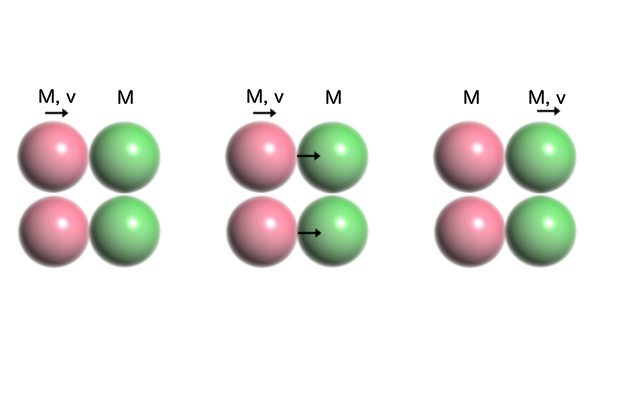
\includegraphics[width = 0.8\textwidth]{ballsExpected.png}
  \caption{The expected result of the collision between the rigid body consisting
  of the red balls and the rigid body consisting of the green balls.
  In the figure M is the mass of the jointly rigid body consisting of
  the two red and green balls respectively. The two bodies collide and energy and momenta is preserved.}
  \label{fig:ballsExpected}
\end{figure}

\begin{figure}[H]
  \centering
  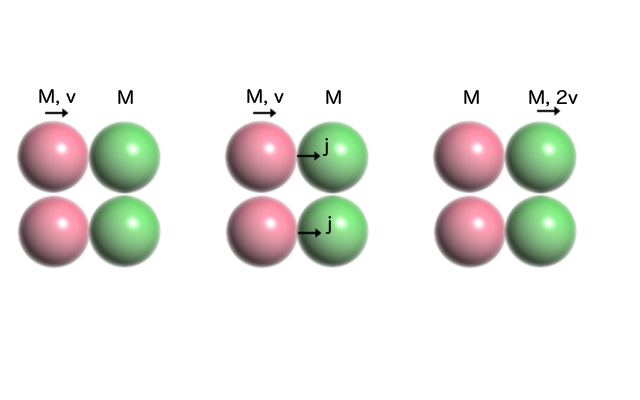
\includegraphics[width = 0.8\textwidth]{ballsNoMassSplit.png}
  \caption{Calculating all impulses in parallel can lead to too high end velocities.
  In the figure M is the mass of the jointly rigid body consisting of
  the two red and green balls respectively. The two bodies collide and energy and momenta is not preserved.}
  \label{fig:noSplit}
\end{figure}

This problem can be remedied by only solving one impulse between a body pair at a time.
This can be achieved as stated above by either backing up time until there
is only one or a few collision(s), and then solve one of them, chosen
arbitrarily. This gives rise to an order dependent system, and is something which
makes for difficult realizations in parallel algorithms. Another approach popularized
by Erin Catto in his Box2D is \textit{Sequential Impulses} which solves the worst interpenetration
on each respective body pair, updates the velocities and reiterates the solution a few times.
One interesting aspect here is that negative impulses are allowed in intermediate
results. However, as the name suggests, it is most suitable for a sequential implementation.
Both of the methods above suggest that only one collision between a body pair should
be solved at a time, which leads to sequential processing. For more details see \cite{catto}.
This method could arguably be parallelized in the sense that each body could be
processed in parallel. However, a different approach is used for this project since
concave collisions is one of the aims for this thesis and extending this method to
handle concave collisions is non-trivial.

\section{Mass splitting}\label{sec:massSplit}
\cite{tonge} describes a parallel constraint based solver
using mass splitting, where objects are split and solved independently and superpositioned
for the final result.

A similar approach would be to split the mass prior to
calculating the impulses by the number of collisions between the two bodies. The
calculated impulses are then applied to the original object. The idea is visualized in figure~\ref{fig:massSplit}, where
we get the expected result.

\begin{figure}[H]
  \centering
  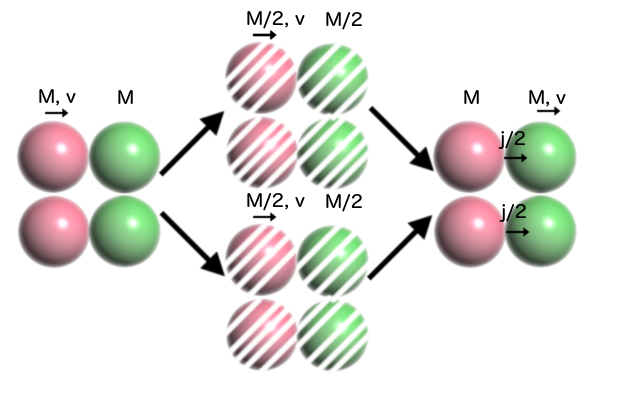
\includegraphics[width = 0.8\textwidth]{ballsMassSplit.png}
  \caption{By mass splitting the objects by the number of interbody collisions
  and applying the resulting impulses to the non-split object we get the expected result.}
  \label{fig:massSplit}
\end{figure}

For this method to be implementable we need to count the number of collisions between
every body pair. This is described in further detail in section~\ref{sec:colMatrix}.

The impulse, defined in equation 2.30, is divided by the number of collisions
 between the bodies, here defined as k. The final modification to
$\vec{j}$ before applying it to the bodies then becomes the following:

\begin{equation}
  \vec{j}_{mass split} = \frac{\vec{j}}{k}
\end{equation}

While inspired by the mass splitting technique from~\cite{tonge}
this is simply an application of the superposition-principle
of forces.

\section{Collision detection}\label{sec:gridCD}
\subsection{Spatial partitioning}
~\cite{gpugems} suggests spatial partitioning
by ways of a uniform grid for collision detection. This method is especially suitable
for the spherical decomposition since we can select an optimized
grid size for a fixed sphere radius. In addition~\cite{gpugems},~\cite{green} and~\cite{fastnearest} claim that sorting
the collisions by bin index increases memory coherence and overall performance.

\subsection{Parallel Sweep-And-Prune}
Parallel Sweep-And-Prune as investigated by~\cite{gpupipedev}, which in turn is based on~\cite{liu2010}, %Find this source
discusses a single axis Sweep-And-Prune algorithm on the GPU for broadphase collision
detection using bounding boxes and the Separating-Axis-Theorem. For more details
concerning the basics of Sweep-And-Prune, turn to the work of~\cite{SAPPierre}.

\section{Time-stepping schemes}
\cite{Lembcke} describes using Guendelman's time stepping
algorithm. By detecting when the velocity is very small the contact impulses can be
calculated by setting $\epsilon = 0$ in equation~\ref{eq:finalJ}.
Guendelman's time stepping algorithm is provided in pseudocode below, in accordance
to what is described in~\cite{guendelman}.

\begin{algorithm}[H]
  \begin{algorithmic}[1]
  \State DetectCollisions
  \ForAll{collisions with |v| > 0}
    \State calculateImpulses
  \EndFor
  \State applyGravity
  \State updateVelocity
    \ForAll{collisions with |v| <= $\epsilon_v$}
      \State calculateImpulse (with elasticity = 0)
    \EndFor
\end{algorithmic}
\end{algorithm}

\section{Nonconvex collision with stacking}
\cite{guendelman} present in their paper \textit{"Nonconvex Rigid Bodies with Stacking"}
a scenario very similar to what this thesis aim to produce.
While the end results reach high physical accuracy the runtime is not suitable for realtime applications.
 Dropping 500 rings consisting of 320 triangles averaged 3 minutes per frame.

In the same paper~\cite{guendelman} present the Shock Propagation algorithm.
By constructing a contact graph from the static objects in the scene (see figure~\ref{fig:cont})
then solving the objects in contact with the static objects first, followed by changing their
mass making them static and solve the next layer and so forth. This lead to much
higher stability in simulations, but does however introduce a sequential dependency
since each level of the graph needs to be processed before the next.

\begin{figure}[H]
  \centering
  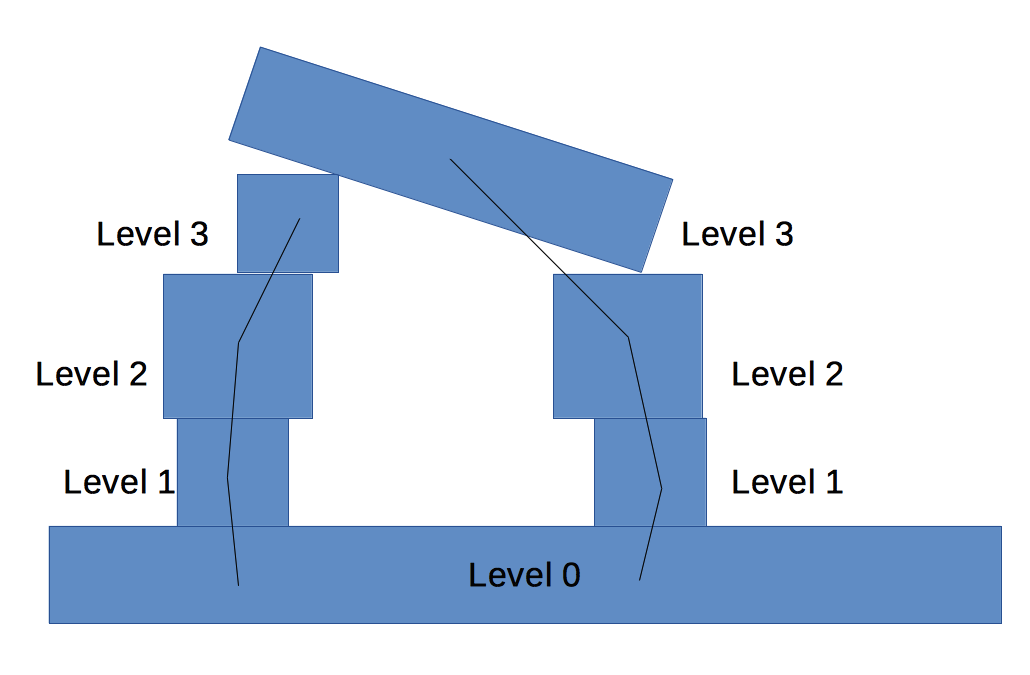
\includegraphics[width = 0.8\textwidth]{shock.png}
  \caption{Contact graph traversing from the static ground upwards. Each box
  represents an object and the large rectangular block at the bottom of the
  image represents a static ground. The distance is measured, as in how many collisions away from the static ground each object is. Each object is assigned a level based on this distance.}
  \label{fig:cont}
\end{figure}

\section{Hierarchical Approximate Convex Decomposition}
A popular method for collision detection of complex concave objects
are convex decomposition. Reasons for the popularity of the method may be its relative
simplicity in theory. Dividing the concave model into convex subsets
can give composite shapes that are concave, yet still work with the
traditional collision detection and response models since they work on convex
sub-shapes. In figure~\ref{fig:hacdSimple} an initially concave shape has
been subdivided in smaller convex shapes. Creating composite shapes in a physics
engine is fairly straightforward as each submodel contributes to the inertia and
mass of the object. The previous collision shape of each object can be used, or a new collision
shape for the whole object can be recalculated. The forces of each submodel
contribute to the movement of the whole model instead of the submodel itself.
There are some automatic methods for convex decompositions, among them hierarchical
 approximate convex decomposition (HACD) developed by~\cite{mamou}.

\begin{figure}[H]
  \centering
  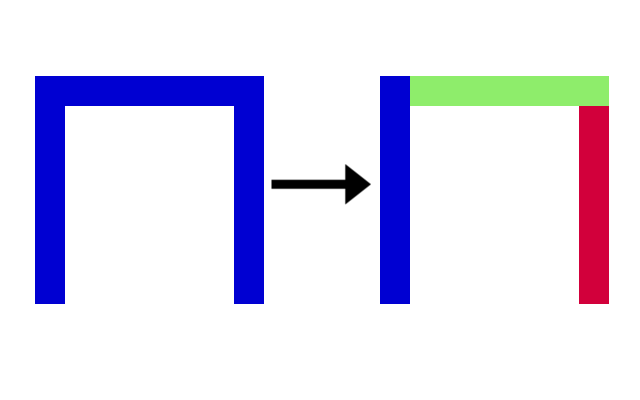
\includegraphics[width = 0.8\textwidth]{hacdSimple.png}
  \caption{The basic idea behind HACD, subdividing a concave shape into smaller convex ones.}
  \label{fig:hacdSimple}
\end{figure}

\cite{HACD} investigated the use of HACD and found it produced fewer hulls
than previous methods while still approximating the original objects well.
Mamou is currently working on a newer version of HACD called
V-HACD, which among other things includes GPU acceleration.
